\subsubsection{Cours}

Le cours est pris de la partie $1$ de \url{https://maths-olympiques.fr/wp-content/uploads/2017/09/combi.pdf}.


\subsubsection{Comptage}


\begin{exo}
Combien d'anagrammes de "DENOMBREMENT" existe-t-il ?
\end{exo}


\begin{exo}
Dénombrer les différentes figures de poker possible / On considère un jeu de classique de 52 cartes.
\begin{itemize}
\item Combien existe-t-il de mains de 5 cartes avec exactement une reine ?
\item Avec au moins une reine ?
\item Avec exactement une figure royale ? (une reine ou un roi)
\item Avec exactement deux reines ?
\item Avec un brelan ? (un full est un brelan mais un carré n'en est pas un)
\item Avec un full ?
\end{itemize}
\end{exo}


\begin{exo}
On a $n$ droites dans le plan en position générale (2 droites ne sont jamais parallèles et 3 droites jamais concourantes en un même point). Combien de triangles forment-elles ?
\end{exo}


\begin{exo}
On a une grille de taille $n \times m$. Une fourmi débute en $(0;0)$ et veut rejoindre la case $(n;m)$, mais elle ne peut aller que vers le haut ou la droite. Combien de chemins peut-elle emprunter ?
\end{exo}


\begin{exo}
Soit $n,k\in \N^*$, calculer le nombre de solutions $(a_1,\dots a_k)\in (\N^*)^k$ de $a_1+\dots +a_k=n$. Calculer le nombre de solutions $(a_1,\dots a_k)\in \N^k$ de $a_1+\dots +a_k=n$.
\end{exo}


\begin{exo}
Démontrer de manière combinatoire que :
$$\binom{n}{k}=\binom{n}{n-k}$$
\end{exo}


\begin{exo}
Démontrer de manière combinatoire que
$$ \sum_{k = 0}^{n}{\binom{n}{k}} = 2^n $$
\end{exo}


\begin{exo}
Démontrer de manière combinatoire que
$$k \cdot \binom{n}{k} = n \cdot \binom{n-1}{k-1}$$
Puis
$$\sum_{k = 0}^{n}{k \cdot \binom{n}{k}} = n \cdot 2^{n-1}$$
\end{exo}


\begin{exo}[Identité de Vandermonde]
Démontrer de manière combinatoire que
$$\sum_{k = 0}^{n}{\binom{a}{k} \cdot \binom{b}{n-k}} = \binom{a+b}{n}$$
\end{exo}


\begin{exo}
Démontrer de manière combinatoire que :
$$\sum_{k = 0}^{n}{\binom{n}{k} \cdot \binom{k}{m}} = 2^{n-m}{\binom{n}{m}}$$
\end{exo}


\begin{exo}
(Dur) On considère une grille triangulaire obtenue en divisant un triangle équilatéral de côté $n$ en $n^2$ triangles équilatéraux de côté 1. Déterminer le nombre de parallélogramme qui apparaissent sur cette grille.
\end{exo}


\subsubsection{Pot-pourri}

\begin{exo}
\begin{enumerate}
\item $4$ points sont sur un cercle. Montrer qu’il existe un demi-cercle (bords compris) qui contient $3$ de ces points.
\item $5$ points sont sur une sphère. Montrer qu’il existe une demi-sphère (bords compris) qui contient $4$ de ces points.
\end{enumerate}
\end{exo}

\begin{exo}
Le pays de Cocagne compte $n$ de villes, où $n > 3$ est un entier impair. Les distances entre villes sont deux à deux distinctes. Un jour, chaque maire se rend dans la ville la plus proche de la sienne.

Montrer qu’il y a une ville qu’ont visité au moins deux maires.
\end{exo}

\begin{exo}
On a un quadrillage de taille $3 \times 7$. Chaque case est coloriée en blanc ou en noir. Montrer qu'il existe un rectangle qui a ses 4 sommets de même couleur (une case unique n'est pas considérée comme un rectangle).
\end{exo}

\begin{exo}
On donne $2n$ points dans l'espace. On trace au total $n^2+1$ segments entre ces points. Montrer qu'il y a au moins un ensemble de trois points reliés deux à deux.
\end{exo}

\begin{exo}
Considérons un polyèdre à $S$ sommets, $A$ arêtes et $F$ faces, ne possédant pas $4$ sommets coplanaires. Montrer que
$$S+F = A+2$$
\end{exo}

\begin{exo}
On considère un polyèdre à $20$ faces triangulaires. Combien a-t-il d'arêtes et de sommets ?
\end{exo}

\begin{exo}
En arrivant à Valbonne, chaque élève a au plus 3 amis. Pour qu'ils apprennent à se connaître, les animatheux veulent les séparer en deux groupes de manière à ce que chaque élève ait au plus un ami dans son groupe. Cela est-il possible ?
\end{exo}


\begin{exo}[Difficile]
Soient $m,n\ge 2$ deux entiers. Alice et Bob jouent au jeu dangereux suivant : ils ont devant eux une tablette de chocolats constituée de $m\times n$ carrés, celui en bas à gauche étant empoisonné. Alice commence à jouer et les deux joueurs alternent ensuite. À chaque tour, le joueur dont c'est le tour choisit un des carrés restant et mange ce carré ainsi que tous les carrés au-dessus et à sa droite. Le perdant est le joueur qui mange le carré empoisonné. Qui a une stratégie gagnante ?
\end{exo}


\begin{sol}
Le mot "DENOMBREMENT" possède $n=12$ lettres, donc à priori on pourrait penser qu'il possède $n!$ anagrammes. Cependant, parmi les $n!$ façons de permuter les lettres, on en compte certaines plusieurs fois car certaines lettres apparaissent plusieurs fois dans le mot. Ces lettres sont le "E" qui apparaît $3$ fois, le "N" qui apparaît $2$ fois et le "M" qui apparaît aussi $2$ fois. Ainsi, à chaque permutation des lettres, on retrouve le même anagramme en échangeant les "E", les "N" ou les "M" entre eux. Ainsi, un même anagramme correspond à
$$3!\text{ (permutations des "E") }\cdot 2!\text{ (permutations des "N") }\cdot 2!\text{ (permutations des "M") }=24$$
permutations. Le nombre d'anagrammes de "DENOMBREMENT" est donc
$$\frac{12!}{24}=19958400.$$
\end{sol}

\begin{sol}
\begin{itemize}
\item On a $4$ cartes possibles pour la reine, puis on choisit les $4$ autres cartes de la main parmi $48$ cartes qui ne contiennent pas de reine : $4 \cdot \binom{48}{4}$.
\item On compte cette fois-ci toutes les mains possibles : $\binom{52}{5}$ et toutes les mains avec aucune reine : $\binom{48}{5}$. On soustrait le nombre de mains sans reine au nombre de mains total pour avoir ceux avec au moins une reine, ainsi la réponse est : $\binom{52}{5} - \binom{48}{5}$.
\item Cette fois-ci une à $8$ choix pour la carte avec du roi ou de la reine, puis on pioche les $4$ autres cartes de la main dans les cartes restantes. Ainsi on a : $8 \cdot \binom{44}{4}$.
\item Cette fois-ci on choisit juste nos deux reines parmi les 4 reines possibles, puis on complète comme précédemment : $\binom{4}{2} \cdot \binom{48}{2}$.
\item On commence par choisir la valeur parmi les $13$ possibilités dont sera composée le brelan, puis on choisit les $3$ cartes parmi les $4$ de cette valeur que l'on utilise pour le brelan. Finalement, on choisit $2$ autres cartes parmi les $48$ restantes, ce qui fait un total de $13\cdot \binom43\cdot\binom{48}2$.
\item Pour faire un full, on choisit deux valeurs, celle du brelan et celle de la paire, ce qui fait un total de $13\cdot 12$ possibilités. Enfin, on choisit quelles trois cartes on prend parmi les $4$ de la valeur choisie pour le brelan, et quelles $2$ cartes on prend parmi les $4$ de la valeur choisie pour la paire, ce qui fait au total $13\cdot 12\cdot \binom 43\cdot\binom 42$ possibilités.

\end{itemize}
\end{sol}

\begin{sol}
Un triangle est simplement la donnée de trois droites qui forment ses côtés. Comme il n'y a pas de droites parallèles ni de triplet de droites concourantes, chaque choix de trois droites forme bien un triangle. Ainsi, le nombre de triangles est $\binom n3$.
\end{sol}

\begin{sol}
Quand la fourmi arrive en $(n;m)$, elle a effectué $n$ déplacement vers la droite et $m$ déplacement vers le haut. On considère la suite de nos déplements vers la droite par exemple. Il faut alors trouver comment on positionne nos $m$ déplacements vers le haut sur tous nos déplacements totales, on a : $\binom{n+m}{m}$ chemins possibles.
Mais on peut aussi faire le raisonnement avec $n$ et on a : $\binom{n+m}{n} $ qui vaut bien $\binom{n+m}{m}$.
\end{sol}

\begin{sol}
\begin{enumerate}
\item On dispose $n$ objets en ligne. On cherche à découper cette ligne en $k$ parties avec au moins un élément chacune. En effet, si les tailles de chacune des parties (de gauche à droite) sont $a_1,\ldots,a_k$, ceci revient à choisir un $k$-uplet d'entiers strictement positifs de somme $n$. Mais on peut aussi chercher le nombre de découpages en remarquant qu'un tel découpage revient à placer $k-1$ "barres" entre certains des $n$ objets qui définissent la frontière entre deux parties. On ne peut pas placer deux barres au même endroit puisque les parties doivent contenir au moins $1$ élément. Mais il y a $n-1$ emplacements possibles pour les barres (entre deux éléments consécutifs parmi les $n$), ce qui fait un total de $\binom{n-1}{k-1}$ solutions.
\item Cette fois-ci, l'argument de la question précédente ne marche plus aussi bien puisque l'on peut placer deux "barres" au même endroit. Mais cette question revient en fait à la question précédente: si l'on ajoute $1$ à chacun des $a_i$, alors l'énoncé revient à trouver le nombre de solutions $(a_1,\ldots,a_k)\in(\N^*)^k$ tels que $a_1+\ldots+a_k = n+k$. Ainsi, par la question précédente, le nombre de solutions est $\binom{n+k-1}{k-1}$.
\end{enumerate}
\end{sol}

\begin{sol}
On compte le nombre de manières de choisir $k$ éléments parmi $n$. Par définition, cette valeur vaut $\binom nk$. Mais on peut aussi décider des $n-k$ éléments que l'on ne choisit pas parmi les $n$, et par conséquent cette valeur vaut aussi $\binom n{n-k}$.
\end{sol}

\begin{sol}
On peut remarquer que ce que l'on cherche à montrer est simplement le développement en binôme de Newton de $(1+1)^n$. De manière combinatoire, on peut remarquer que le côté gauche correspond au nombre de manières de choisir un entier $k$ entre $0$ et $n$, puis de choisir $k$ éléments parmi $n$, c'est-à-dire le nombre de manières de choisir une partie des $n$ éléments (de taille quelconque). Mais on peut aussi décider, pour chacun des $n$ éléments, de le prendre ou non, ce qui fait un total de $2^n$ possibilités pour choisir une partie des $n$ éléments.
\end{sol}

\begin{sol}
On compte de deux manières différentes le nombre de façons de choisir $k$ personnes parmi $n$, une d'entre elles étant un chef. D'un côté, on peut choisir les $k$ personnes puis le chef, ce qui fait $k\binom nk$ possibilités. Mais on peut aussi choisir le chef (entre $n$ possibilités), puis les $k-1$ autres personnes à choisir parmi les $n-1$ personnes restantes, ce qui fait $n\binom{n-1}{k-1}$ possibilités.

On peut montrer la deuxième égalité en appliquant la première ainsi que l'exercice précédent. Mais on peut aussi procéder de manière combinatoire: le côté gauche correspond au nombre de manières de choisir une partie des $n$ personnes, dont un chef, ce que l'on peut aussi compter en choisissant un chef (entre $n$ possibilités), puis une partie des $n-1$ autres personnes (ce qui fait $2^{n-1}$ possibilités comme dans l'exercice précédent).
\end{sol}

\begin{sol}
On commence par déterminer la signification combinatoire du côté droit: c'est le nombre de manières de choisir $n$ éléments parmi $a+b$. Ceci fait penser à séparer les $a+b$ éléments en les $a$ premiers et les $b$ derniers. On peut aussi dénombrer cette valeur en déterminant le nombre d'éléments $k$ à choisir parmi les $a$ premiers, puis les $k$ éléments parmi les $a$ et les $n-k$ autres parmi les $b$ derniers, ce qui donne le côté gauche.
\end{sol}

\begin{sol}
Prenons un ensemble $A$ à $n$ éléments. On va compter le nombre de manières de choisir un sous-ensemble $B$ à $m$ éléments ainsi qu'un sous-ensemble intermédiaire $C$ (c'est-à-dire qui contient $B$). D'un côté, on peut d'abord choisir $B$ avec $\binom nm$ possibilités, puis choisir lesquels des $n-m$ éléments hors de $B$ on rajoute à $C$, ce qui fait $2^{n-m}$ possibilités et donc on retrouve bien le terme de droite.

Sinon, on peut d'abord choisir la taille $k$ de l'ensemble $C$, puis l'ensemble $C$ lui-même avec $\binom nk$ possibilités, et l'ensemble $B$ contenu dans $C$ ce qui fait $\binom km$. Ainsi, on retrouve le terme de gauche et les deux côtés sont bien égaux.
\end{sol}

\begin{sol}
Remarquons qu'un parallélogramme dans le triangle peut avoir une de trois orientations, donnée par le côté du triangle qui n'est pas parallèle aux côtés du parallélogramme. Il y a le même nombre de parallélogrammes de chaque orientation donc il suffit de compter ceux dont aucun côté n'est parallèle au côté bas du triangle (voir figure ci-dessous). Un tel parallélogramme est défini par quatre droites qui proviennent de quatre points sur le côté bas du triangle. Tout choix de quatre points sur les $n+1$ points en bas du triangle définit alors un unique parallélogramme (comme sur la figure). Mais il faut faire attention car on n'a pas compté les parallélogrammes qui touchent le côté bas du triangle, qui correspondent eux au cas où les deuxième et troisième points sont confondus. Ce cas-ci correspond alors au choix de trois points sur le côté bas du triangle et le nombre de parallélogrammes dans le triangle est (en n'oubliant pas de multiplier par $3$ pour tenir compte de l'orientation) :
$$3\left(\dbinom{n+1}4+\dbinom{n+1}3\right)=3\dbinom{n+2}4$$
par la formule de Pascal.

\begin{center}
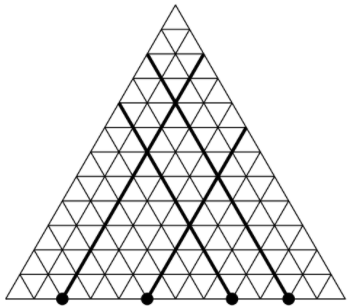
\includegraphics[]{B-23-PM-0.PNG}
\end{center}
\end{sol}

\begin{sol}
\begin{enumerate}
\item Considérons un des quatre points $A$ ainsi que le point diamétralement opposé $A'$. Ces deux points définissent deux demi-cercles contenant $A$ parmi lesquels les $3$ autres points sont répartis. Par le principe des tiroirs, un de ces demi-cercles contient $2$ de ces points, ce qui fait $3$ points en comptant $A$.
\item Considérons deux des cinq points $A$ et $B$ ainsi que le cercle $\mathcal{C}$ passant par ces deux points et dont le centre est le centre de la sphère. Comme dans la question précédente, les trois derniers points sont répartis sur les deux demi-sphères délimitées par $\mathcal{C}$, qui contiennent aussi $A$ et $B$. Par le principe des tiroirs, une des demi-sphères contient $2$ des trois autres points, et en comptant $A$ et $B$, contient au moins $5$ des points.
\end{enumerate}
\end{sol}

\begin{sol}
Soit $i(M)$ la distance parcourue par le maire $M$. Si l'on a deux maires $M,M'$ qui vérifient $i(M)=i(M')$, alors comme toutes les distances entre les villes sont distinctes, ceci signifie que les deux maires ont parcouru le même chemin en sens inverse et sont allés chacun dans la ville de l'autre. On dit alors que les deux maires ont fait un \textit{échange}.

Comme il y a un nombre impair de villes, tous les maires ne peuvent pas avoir fait un échange, soit alors $M$ le maire n'ayant pas fait d'échange tel que $i(M)$ soit maximal. Alors aucun autre maire n'a pu visiter la ville de $M$: si $M'$ est un autre maire, soit il a fait un échange, donc pas avec $M$ puisque $M$ n'a pas fait d'échange, soit il vérifie $i(M')<i(M)$. Mais s'il était allé dans la ville de $M$, alors les villes de $M$ et $M'$ seraient reliées, et comme chaque maire va dans la ville la plus proche, on aurait $i(M)\le i(M')$, absurde.

Ainsi, comme il y a une ville non visitée, il y a forcément une ville visitée deux fois.
\end{sol}

\begin{sol}
Un rectangle a ses $4$ sommets de même couleur si deux colonnes ont deux points de la même couleur à la même hauteur. On calcule le nombre de possibilités de colonnes complètement différentes et qui ont au plus deux points d'une même couleur. On a donc $2 \cdot \binom{3}{2} = 6$ possibilités de colonnes (on regarde comment on prend les deux points d'un certaine couleur pour les deux couleurs). Si les $3$ points de la dernière colonne, c'est gagné, sinon par principe des tiroirs, il y aura au moins deux colonnes identiques, donc c'est aussi gagné.
\end{sol}

\begin{sol}
On procède par récurrence pour montrer que si l'on a $2n$ points reliés par des segments sans que trois points soient reliés deux à deux, alors il y a au plus $n^2$ segments. Pour $n=1$, l'énoncé est trivial.

Supposons le résultat vrai au rang $n$ et montrons le au rang $n+1$. Soient donc $2n+2$ points reliés par des segments sans que trois points soient reliés deux à deux. S'il n'y a aucun segment, on a démontré le résultat voulu. Sinon, il existe deux points $A$ et $B$ reliés par un segment. Alors entre les $2n$ points restants, l'hypothèse de récurrence nous assure qu'il y a au plus $n^2$ segments. Mais si l'on considère les segments issus de $A$ où $B$ vers un de ces $2n$ points, il ne peut pas y en avoir plus de $2n$, car sinon par le principe des tiroirs un des $2n$ points $C$ est relié à $A$ et $B$ et les points
$A,B,C$ sont reliés deux à deux. Mais alors le nombre de segments dans le plan vaut au plus
$$n^2\text{ (entre les 2n points)}+2n\text{ (de A ou B vers les 2n points)}+1\text{ (entre A et B)}$$
$$=(n+1)^2$$
ce qui conclut.
\end{sol}


\begin{sol}
On procède par récurrence sur le nombre de sommets. Si $S=4$ (le minimum pour un polyèdre), alors on a un tétraèdre et $A=6$ et $F=4$ donc la propriété est vérifiée. Supposons le résultat vrai pour $S=n$ sommets et considérons un polyèdre à $S=n+1$ sommets.

Soit $X$ un de ces sommets, et soit $a$ le nombre d'arêtes partant de $X$. Si l'on supprime $X$ et les arêtes correspondantes, on supprime aussi $a$ faces dont $X$ est un sommet, et on rajoute une face dont les sommets sont les voisins de $X$. Par l'hypothèse de récurrence appliquée au nouveau polyèdre, on a
$$(S-1)+(F-a+1) = (A-a)+2$$
soit
$$S+F=A+2.$$
\end{sol}


\begin{sol}
Notons $S,A,F$ les nombres de sommets, arêtes, faces respectivement, afin que $F=20$. On va procéder par double comptage. On compte les couples $(a,f)$ où $a$ est une arête et $f$ est une face dont $a$ est un côté. Chaque arête appartient à deux faces donc ce nombre vaut $2A$. Mais comme les faces sont triangulaires, chaque face possède trois côtés donc ce nombre faut aussi $3F=60$. On en déduit $A=30$.

Maintenant que l'on a $A$ et $F$, on pense à la formule d'Euler (l'exercice précédent) pour trouver $S$. On a
$$S=A+2-F=30+2-20$$
d'où $S=12$.
\end{sol}


\begin{sol}
C'est en effet possible. On peut résoudre ce problème à l'aide d'un monovariant. Pour ceci, on commence par séparer les élèves en deux groupes de manière arbitraire (par exemple tout le monde dans un seul groupe). On définit $M$ le malheur des élèves, qui est la somme sur tous les élèves, de leur nombre d'amis dans leur groupe.

À tout moment, supposons qu'un élève $A$ ait au moins deux amis $B,C$ dans son groupe. Si l'on décide de le changer de groupe, alors $A$ perd deux amis et en regagne au plus $1$. De plus, il a potentiellement un ami dans l'autre groupe qui lui gagne un ami, et $B,C$ perdent tous les deux un ami. Alors la nouvelle valeur de $M$ est
$$\le M -2+1\text{ (pour A) }+1\text{ (pour l'ami de A dans le deuxième groupe) }-2\text{ (pour B et C) }=M-2.$$
Ainsi, la valeur de $M$ ne fait que diminuer strictement. Si l'on continue à faire des échanges comme ceci, au bout d'un moment on ne pourra plus continuer car $M$ ne peut pas être négatif. Dans cette situation, chaque élève a au plus $1$ ami dans son groupe puisque sinon on pourrait l'échanger pour faire diminuer $M$, ce qui conclut.
\end{sol}


\begin{sol}
Commençons par remarquer qu'un des deux joueurs a forcément une stratégie gagnante. Supposons par l'absurde que ce soit Bob. Alors si Alice commence par manger le carré en haut à droite de la tablette, Bob peut mettre en place une stratégie qui assure sa victoire, et qui commence par manger un certain carré $A$. Mais si Alice commençait par manger le carré $A$ dès le départ, elle pourrait voler la stratégie de Bob et alors avoir une stratégie gagnante, absurde. Ainsi, c'est Alice qui a une stratégie gagnante.
\end{sol}
